% ---
\subsection{Classificação}
% ---

A classificação é uma análise preditiva com o objetivo de estabelecer modelos que possbilitem uma previsão do futuro, permitindo estudar tendências por meio do uso de técnicas estatísticas sobre dados históricos.

\subsubsection{Regressão Linear}


A regressão linear é uma modelagem matemática \footnotemark \footnotetext{modelagem matemática é uma representação em fórmulas matemáticas que tentam descrever ou simular eventos e sistemas reais com o propósito de prever comportamentos} que permite descrever variáveis em função de outras. Segundo \citeonline[p. 44]{HASTIE} ela pode ser representada como
\begin{equation}
  \label{eq:regressao_linear}
  \begin{aligned}
Y &= \hat{\beta_{0}} + \sum_{j=1}^{p} (X_{j}\hat{\beta_{j}}), 
  \end{aligned}  
\end{equation}
onde \begin{math}Y\end{math} representa uma variável dependente contínua, \begin{math}X_{j}\end{math} as variáveis independentes (contínuas, discretas ou binárias). Isto significa que uma certa característica (variável dependente) pode ser descrita por outras (variável independente).

Para ajustar o modelo linear ao conjunto de dados, é possível utilizar diferentes maneiras. Um deles é método dos mínimos quadrados, uma técnica de otimização matemática que visa encontrar ajuste ótimo para um conjunto de dados por meio da minimização a soma dos quadrados das diferenças entre o valor estimado e os dados observados, representado por:

\begin{equation}
  \label{eq:minimos_quadrados}
  \begin{aligned}
G(\beta) &= \sum_{i=1}^{N} (y_{i}-x_{i}^{T}\beta)^{2}, 
  \end{aligned}  
\end{equation}

Assim, nosso problema passar a ser como descobrir \begin{math}\hat{\beta}\end{math} que minimize \ref{eq:minimos_quadrados}. Para calcular \begin{math}\hat{\beta}\end{math}, é possível utilizar a equação:

\begin{equation}
  \label{eq:solucao_minimos_quadrados}
  \begin{aligned}
\hat{\beta} &= (X^{T}X)^{-1}X^{T}y, 
  \end{aligned}  
\end{equation}

onde \begin{math} X \in \mathbb{R}^{N,p} \end{math} X representando uma matriz com cada linha sendo um vetor do conjunto de dados de entrada e \begin{math}y \in \mathbb{R}^{N}\end{math} um vetor que representa os dados de saída \footnotemark \footnotetext{inicialmente, esses dados devem vir do conjunto de treino}

Com a definição de \begin{math}\hat{\beta}\end{math}, é possível determinar uma reta que separa o conjunto de dados.

\begin{figure}[!ht]
\caption{Exemplo de classificação em 2 dimensões.}
\centerline{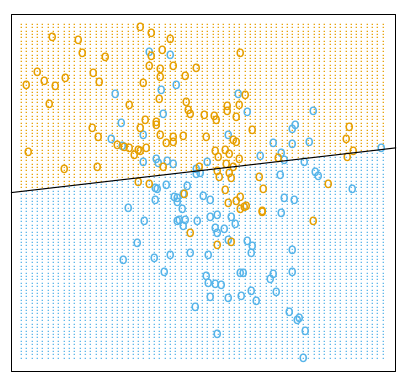
\includegraphics[width=0.5\textwidth]{img/hiperplano}}
\fonte{Extraído de \cite{HASTIE}}
\end{figure}

 As classes estão representadas um variável binária (AZUL = 0, LARANJA = 1), ajustadas por uma regressão linear. A linha que separa os grupos foi definido por \begin{math}x^{T}\hat{\beta} = 0,5\end{math}. A área hachurada em laranja representa o espaço classificado por LARANJA enquanto a área em azul, classificado por AZUL

\subsubsection{Regressão Logística}

Segundo \citeonline[p. 119]{HASTIE}, a regressão logística, assim como a regressão linear, também é um modelo matemático de predição de eventos usada para descrever dados e explicar a relação entre um conjunto de variáveis independentes e uma variável dependente. Contudo, enquanto na regressão linear a variável dependente é contínua, na regressão logística, ela é considerada uma variável categórica. Ela segue uma distribuição Bernoulli\footnotemark \footnotetext{distribuição de Bernoulli é uma modelagem de probabilidade que representa eventos binários cujas ocorrências são tratados como sucesso ou falha. Considerando que a probabilidade de ocorrer um sucesso é \begin{math}p\end{math}, então a probabilidade de ocorrer uma falha é \begin{math}1-p\end{math} } com uma probabilidade \begin{math}p\end{math} desconhecida. Assim, a regressão logística tem como objetivo estimar essa probabilidade \begin{math}p\end{math} desconhecida.

Para estimar essa probabilidade, a regressão logística usa as chances (\emph{odds}) do evento ocorrer em cada variável independente, calculando a taxa dessas chances, dada pela equação:

\begin{equation}
  \label{eq:OR}
  \begin{aligned}
   OR &= \frac{P(sucesso)}{P(fracasso)}
     &= \frac{p}{1-p}.
  \end{aligned}
\end{equation}

Utilizando inferência de estatística, podemos aplicar log em \ref{eq:OR}, ficando com:

\begin{equation}
  \label{eq:t}
  \begin{aligned}
    logit(p) &= ln\left ( \frac{p}{1-p} \right ).
  \end{aligned}
\end{equation}

Tal transformação recebe o nome de logit. Ela é ajustada a função de predição, como numa análise de regressão linear, visto anteriormente. O valor final obtido a partir da função logit é convertido novamente para as chances via a função inversa do logaritmo natural (ou uma função exponencial).

\begin{equation}
  \label{eq:t}
  \begin{aligned}
    logit^{-1}(\alpha) &= \frac{1}{1+e^{-\alpha}} &= \frac{e^{\alpha}}{1+e^{\alpha}}.
  \end{aligned}
\end{equation}

\begin{figure}[!ht]
\caption{Fun\c c\~ao logit}
\centerline{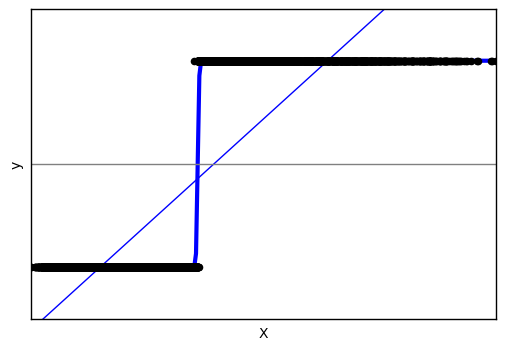
\includegraphics[width=.6\textwidth]{img/logit}}
\fonte{Gerado a partir do script LogisticRegression.ipynb}
\end{figure}


Generalizando com \ref{eq:t1}, \ref{eq:t2} e \ref{eq:t3} , temos:

\begin{equation}
  \label{eq:t1}
  \begin{aligned}
    \log\left ( \frac{P(G = 1 | X = x)}{P(G = K | X = x)} \right ) &= \beta_{10}+\beta_{1}^{T}x
  \end{aligned}
\end{equation}

\begin{equation}
  \label{eq:t2}
  \begin{aligned}
    \log\left ( \frac{P(G = 2 | X = x)}{P(G = K | X = x)} \right ) &= \beta_{20}+\beta_{2}^{T}x
  \end{aligned}
\end{equation}

\begin{equation}
  \label{eq:t3}
  \begin{aligned}
    \log\left ( \frac{P(G = K-1 | X = x)}{P(G = K | X = x)} \right ) &= \beta_{(k-1)0}+\beta_{k-1}^{T}x,
  \end{aligned}
\end{equation}

onde o modelo é composto por K classes e K - 1 transformações logit. Utilizando a inversa da logit, temos:

\begin{equation}
  \label{eq:t4}
  \begin{aligned}
    P(G = k | X = x) &= \frac{\exp \left ( \beta_{k0}+\beta_{k}^{T}x \right )}{1 + \sum_{\ell=1}^{K - 1}\exp \left ( \beta_{\ell0}+\beta_{\ell}^{T}x \right )}, k = 1, ..., K - 1\\
    P(G = K | X = x) &= \frac{1}{1 + \sum_{\ell=1}^{K - 1}\exp \left ( \beta_{\ell0}+\beta_{\ell}^{T}x \right )} .
  \end{aligned}
\end{equation}

Dessa forma, temos com \ref{eq:t4} que a regressão logística estima as changes (odds) como uma variável contínua, mesmo quando a variável dependente que está sendo o objeto de estudo seja uma variável binária. 



\begin{comment} 
\begin{citacao} 
\cite{HASTIE} \end{citacao}
, mas que leva em consideração as probabilidades de ocorrência desses eventos.
\end{comment}

Assim, a regressão logística viabiliza a classificação das observações por meio da probabilidade estimada na categoria estudada.
